% ----------------------------------------------------------
% Metodologia
% 
% ----------------------------------------------------------

\chapter[Pesquisa/Amostragem]{Pesquisa/Amostragem}

Para a pesquisa foi realizado um levantamento de quais informações seriam de suma importância para o projeto, com isso, foi obtido um total de 15 perguntas, dentre elas, múltipla escolha e dissertativa, onde todas as respostas foram obrigatórias. Foi criado um formulário, com base nas perguntas levantadas, para que os estudantes da Universidade Municipal de São Caetano do Sul pudessem respondê-lo.

O formulário ficou disponível para o recebimento de respostas durante 1 semana. Este formulário foi devidamente analisado e validado de forma científica pelo orientador \imprimirorientador.

\section{Tipo de Pesquisa}
A pesquisa que propomos, conforme metodologias descritas em Baptista e Campos (2018), é baseada em pesquisas quantitativas. Essa é uma metodologia que permite desenvolver conclusões gerais das pesquisas e prever resultados, pois ela envolve a coleta de dados que podem ser traduzidos em números para análises posteriores, os dados quantitativos são estruturados e estatísticos. diferente da pesquisa qualitativa, que coleta dados não numéricos para a obtenção de insights. Ela não é estatística e não é estruturada, é fundamentada em dados coletados por meio de um esquema de pergunta do tipo “por quê”. O tipo de pesquisa qualitativa usa gráficos ou tabelas para medir opiniões, pontos de vista e atributos numéricos.
Conforme foi feita a pesquisa quantitativa, conseguimos coletar dados de pessoas que responderam em cada pergunta. Possibilitando desenvolver uma conclusão sobre o nosso projeto e poder decidir de forma assertiva o segmento do projeto para o público alvo.

\section{Público Alvo}
Considerando a população de, aproximadamente, 500 pessoas, é possível concluir que seria necessário considerar uma amostra de, pelo menos, 286 pessoas, com um grau de confiança de 99\% e uma margem de erro de 5\%. Quando realizada, a pesquisa obteve um total de 380 respostas, o que é considerado uma quantidade mais que adequada, descartando qualquer viés que possa induzir ao erro.

    \vspace{\baselineskip}
    \vspace{\baselineskip}
    %\vspace{\baselineskip}
    
\section{Respostas}

\begin{enumerate}

    \item Idade

    A figura 1 descreve a idade das pessoas respondentes da pesquisa.

    \vspace{\baselineskip}
    \begin{center}
        \begin{minipage}{\textwidth}
            %\centering
            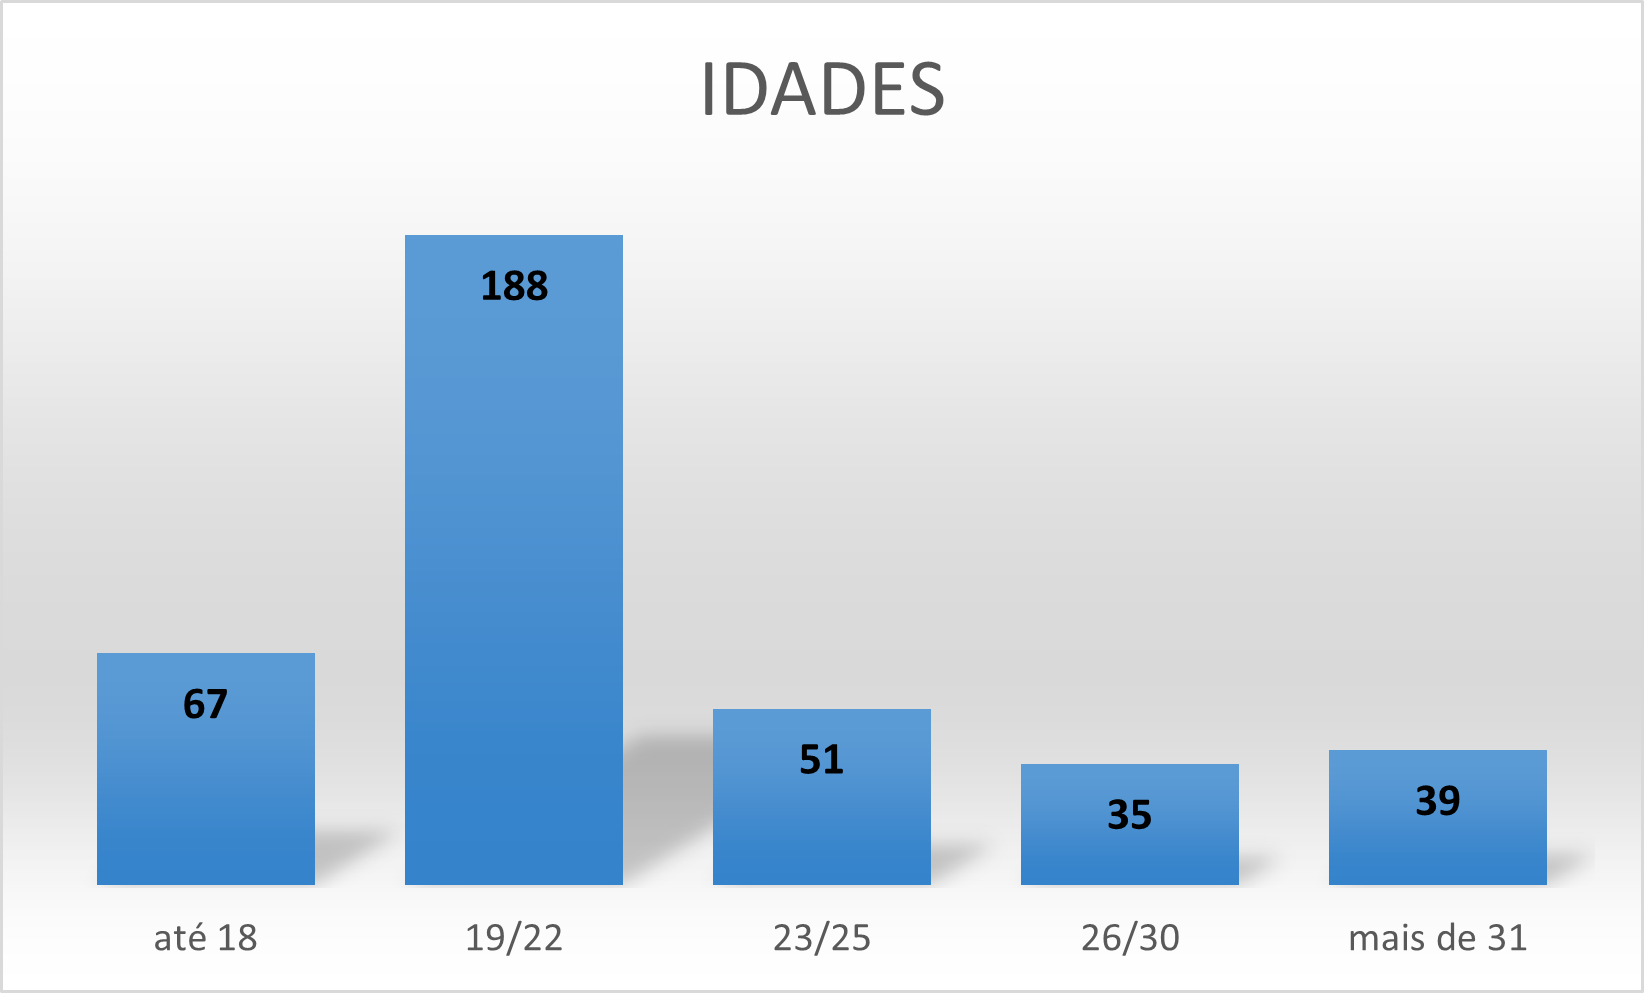
\includegraphics{figs/graph_idade.png}
            \captionof{figure}{Idade}
            \label{fig:graph_idade}
        \end{minipage}        
    \end{center}



    \item Tipo da Cidade

    A figura 2 descreve o tipo da cidade das pessoas respondentes da pesquisa.

    \vspace{\baselineskip}
    \begin{center}
        \begin{minipage}{\textwidth}
            %\centering
            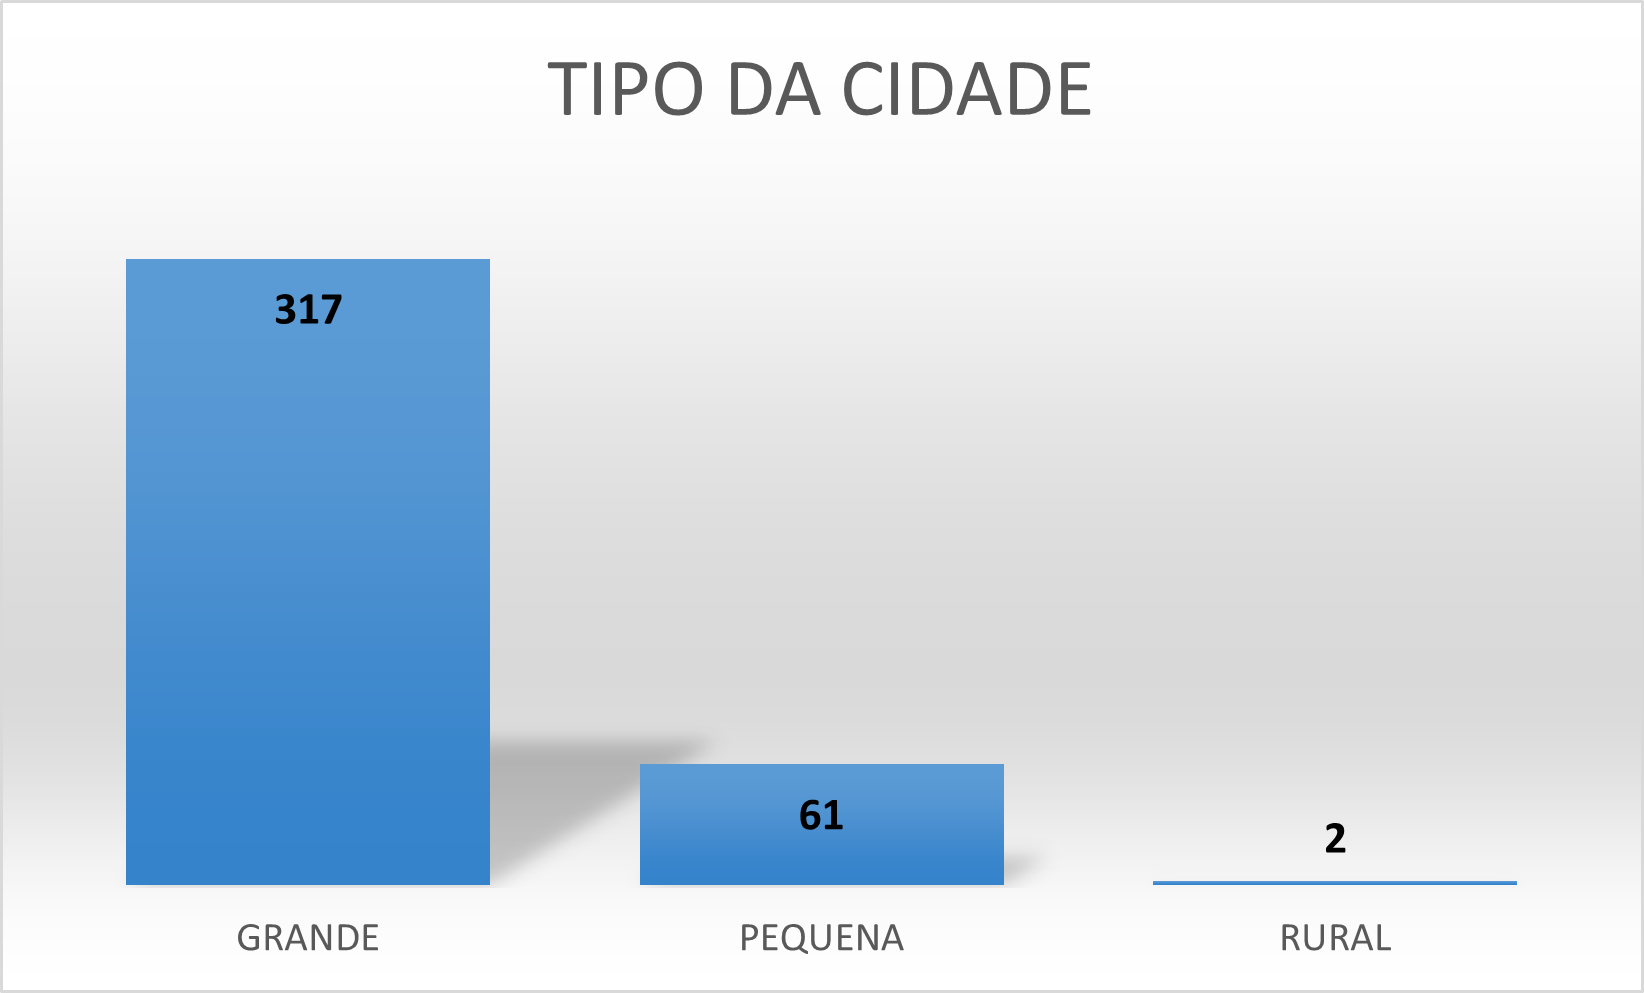
\includegraphics{figs/graph_cidade.png}
            \captionof{figure}{Tipo da Cidade}
            \label{fig:graph_cidade}
        \end{minipage}     
    \end{center}


    \vspace{\baselineskip}
    \vspace{\baselineskip}
    \item Formação

    A figura 3 descreve a formação das pessoas respondentes da pesquisa.

    \vspace{\baselineskip}
    \begin{center}
        \begin{minipage}{\textwidth}
            %\centering
            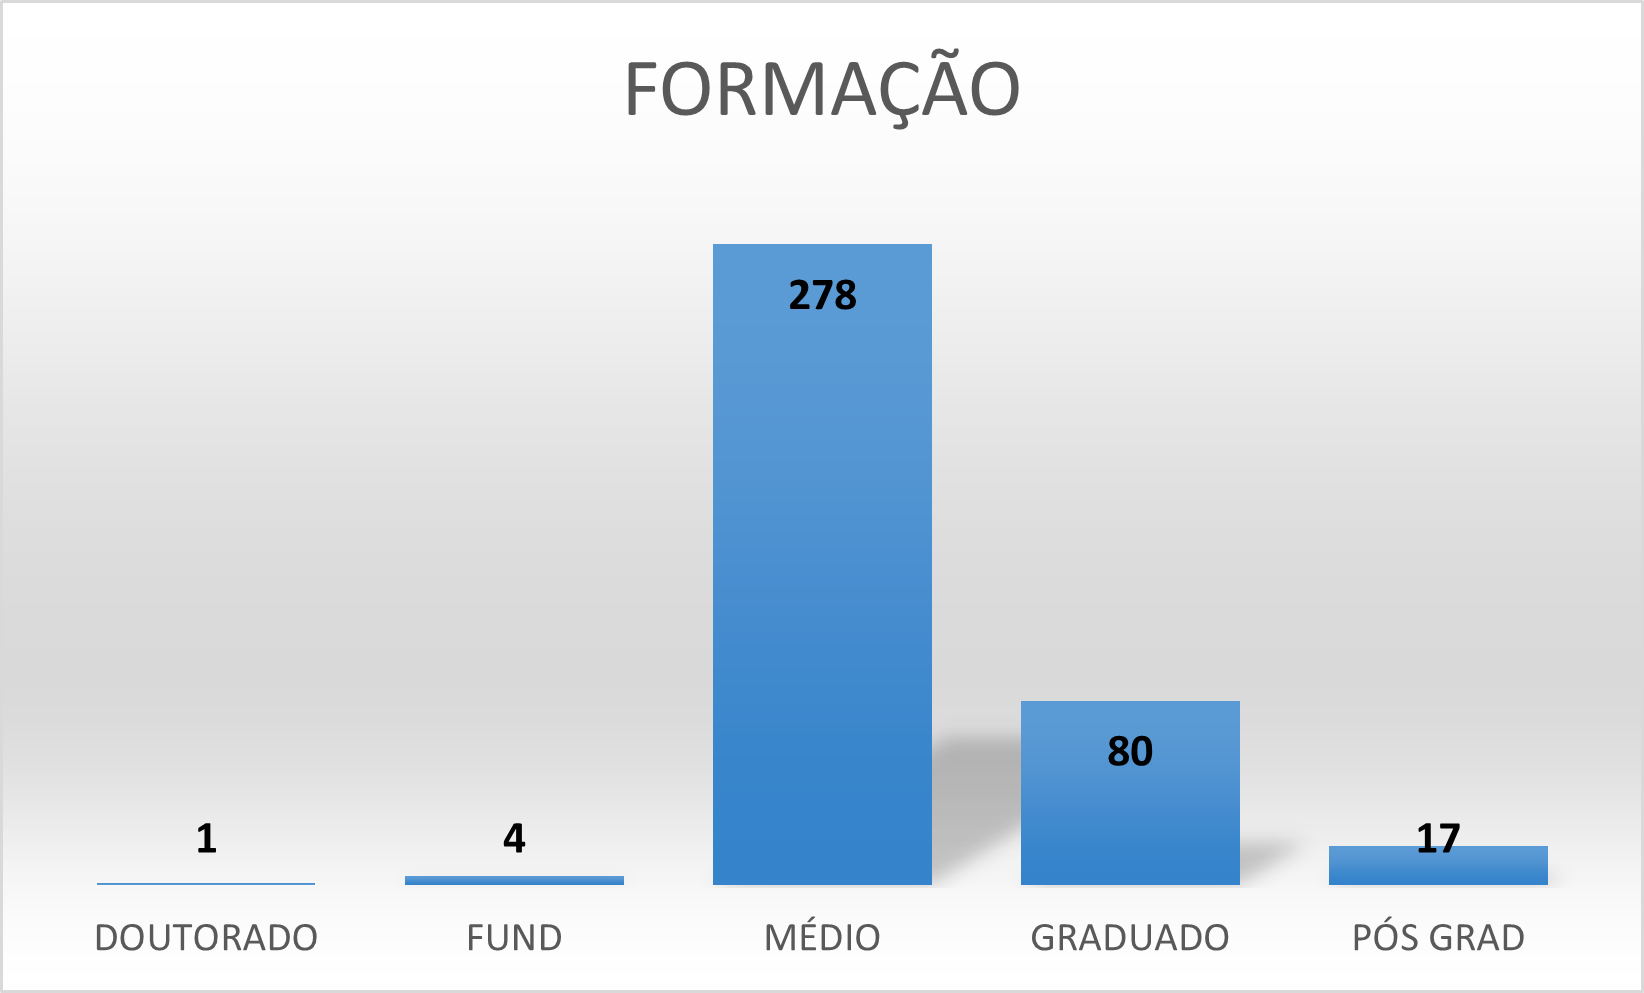
\includegraphics{figs/graph_formacao.png}
            \captionof{figure}{Formação}
            \label{fig:graph_formacao}
        \end{minipage}        
    \end{center}

    \item Renda (em Reais)

    A figura 4 descreve a renda das pessoas respondentes da pesquisa.

    \vspace{\baselineskip}
    \begin{center}
        \begin{minipage}{\textwidth}
            %\centering
            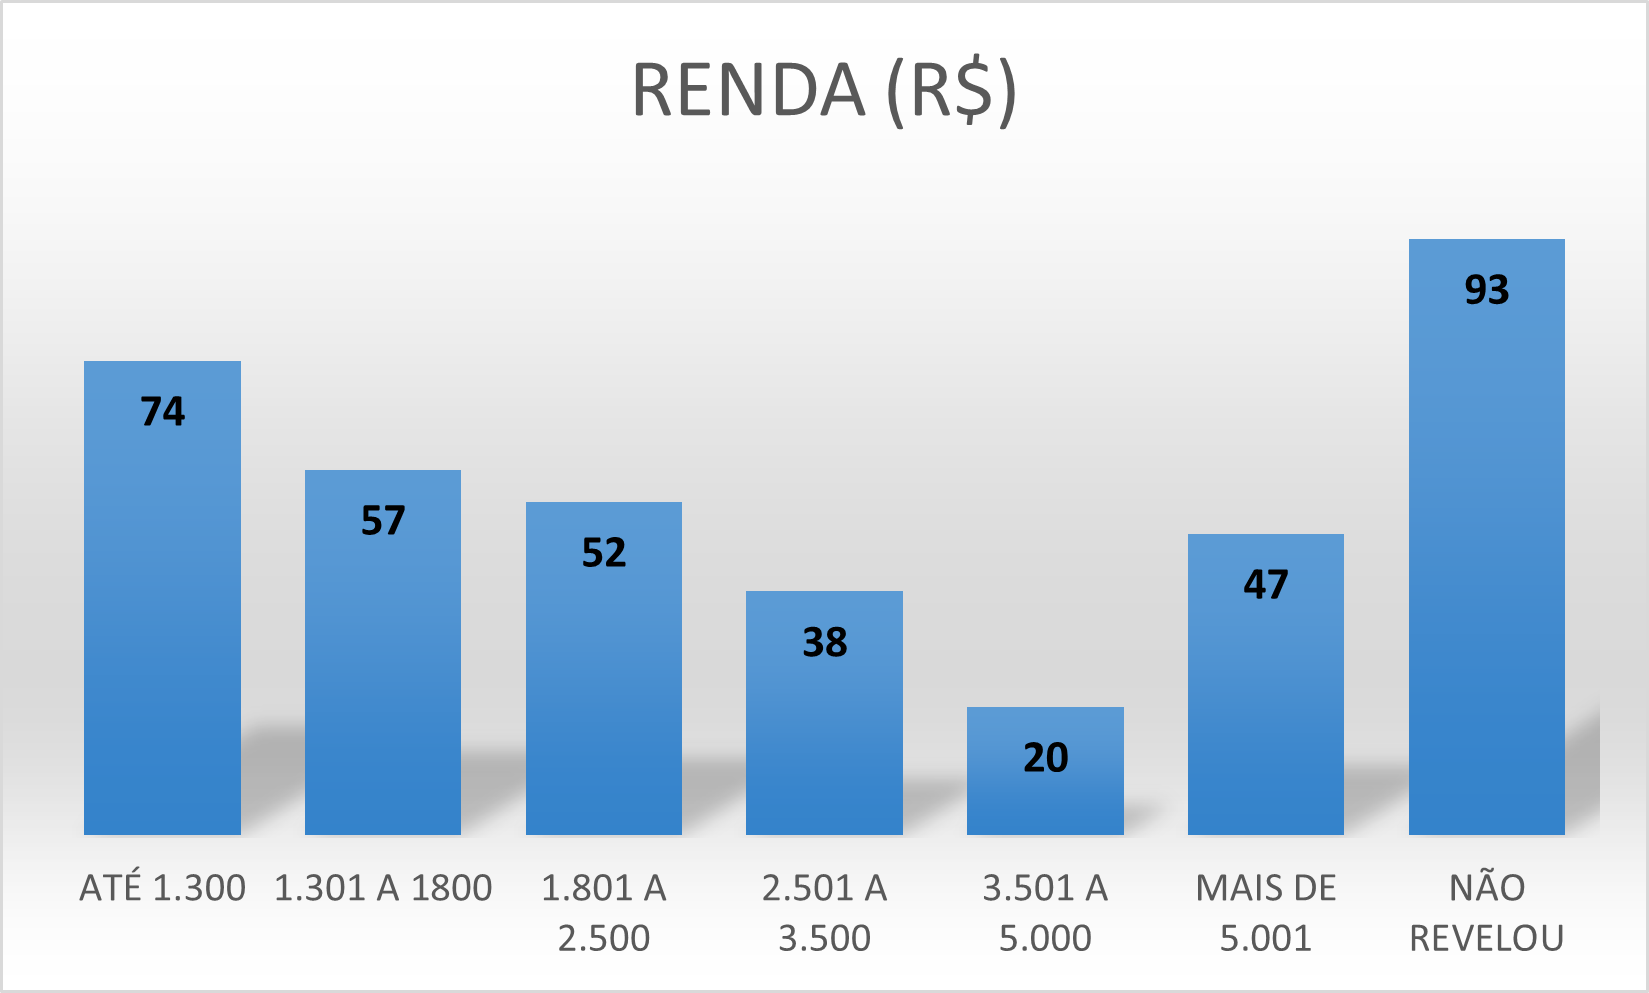
\includegraphics{figs/graph_renda.png}
            \captionof{figure}{Renda}
            \label{fig:graph_renda}
        \end{minipage}        
    \end{center}

    \vspace{\baselineskip}
    \vspace{\baselineskip}
    \vspace{\baselineskip}
    \vspace{\baselineskip}
    \vspace{\baselineskip}
    \item Situação Financeira

    A figura 5 descreve a situação financeira das pessoas respondentes da pesquisa.

    \vspace{\baselineskip}
    \begin{center}
        \begin{minipage}{\textwidth}
            %\centering
            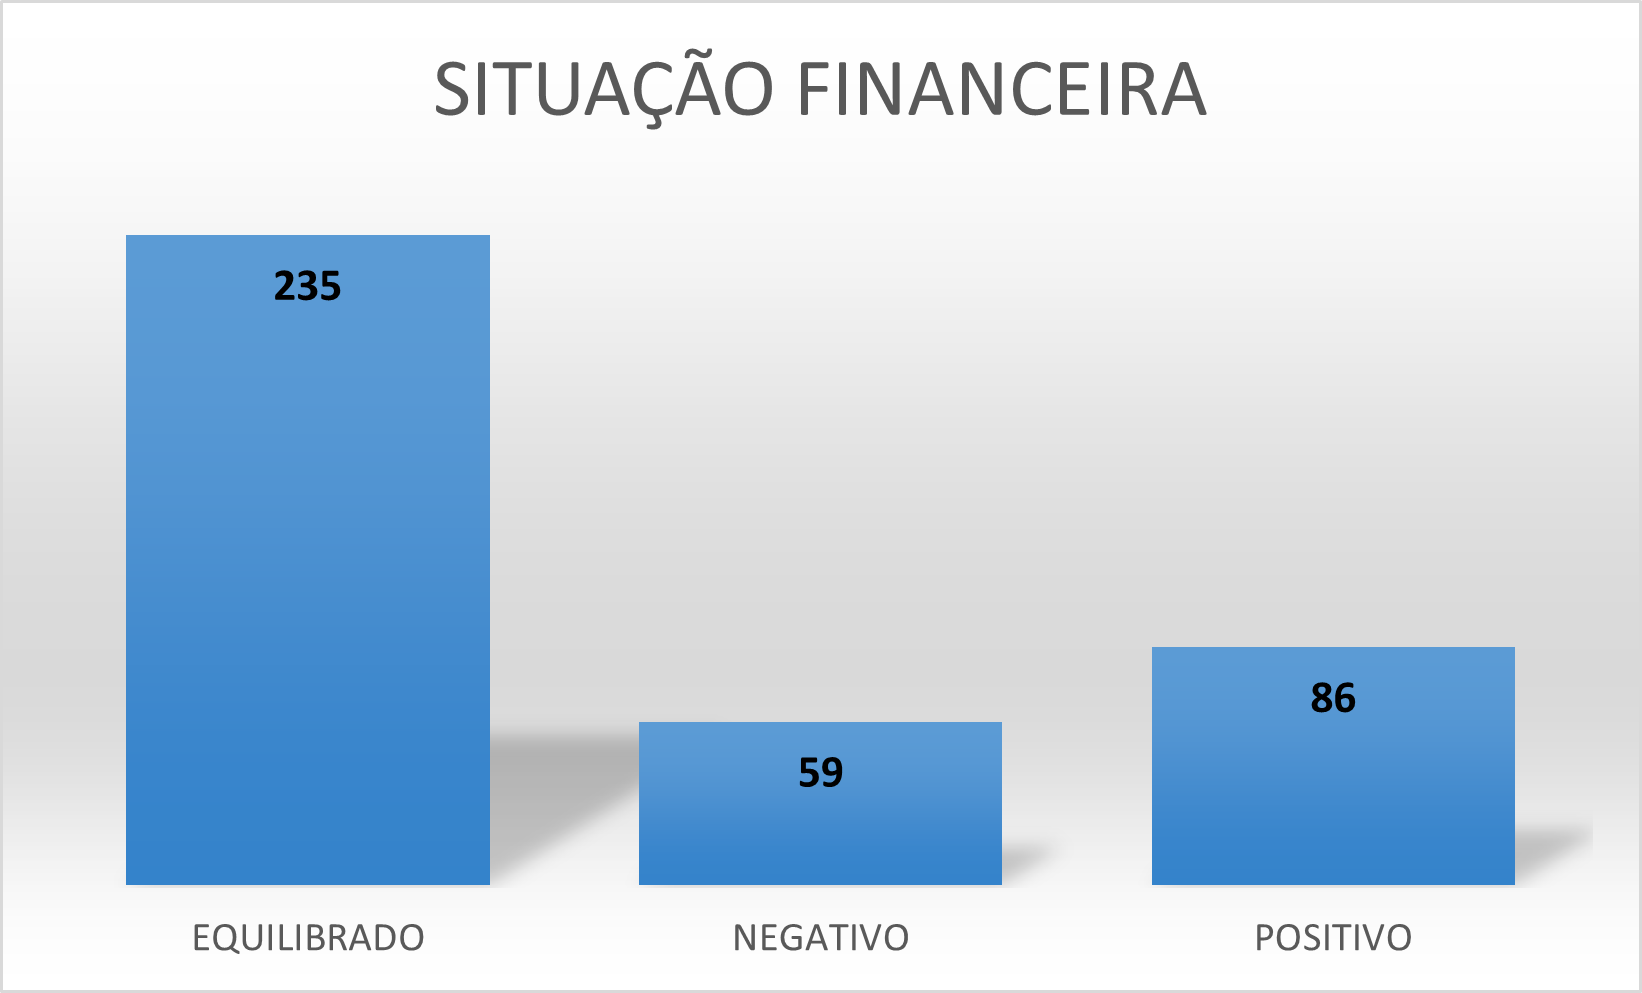
\includegraphics{figs/graph_situacao.png}
            \captionof{figure}{Situação Financeira}
            \label{fig:graph_situacao}
        \end{minipage}        
    \end{center}


    \item Educação Financeira

    A figura 6 descreve a educação financeira das pessoas respondentes da pesquisa.

    \vspace{\baselineskip}
    \begin{center}
        \begin{minipage}{\textwidth}
            %\centering
            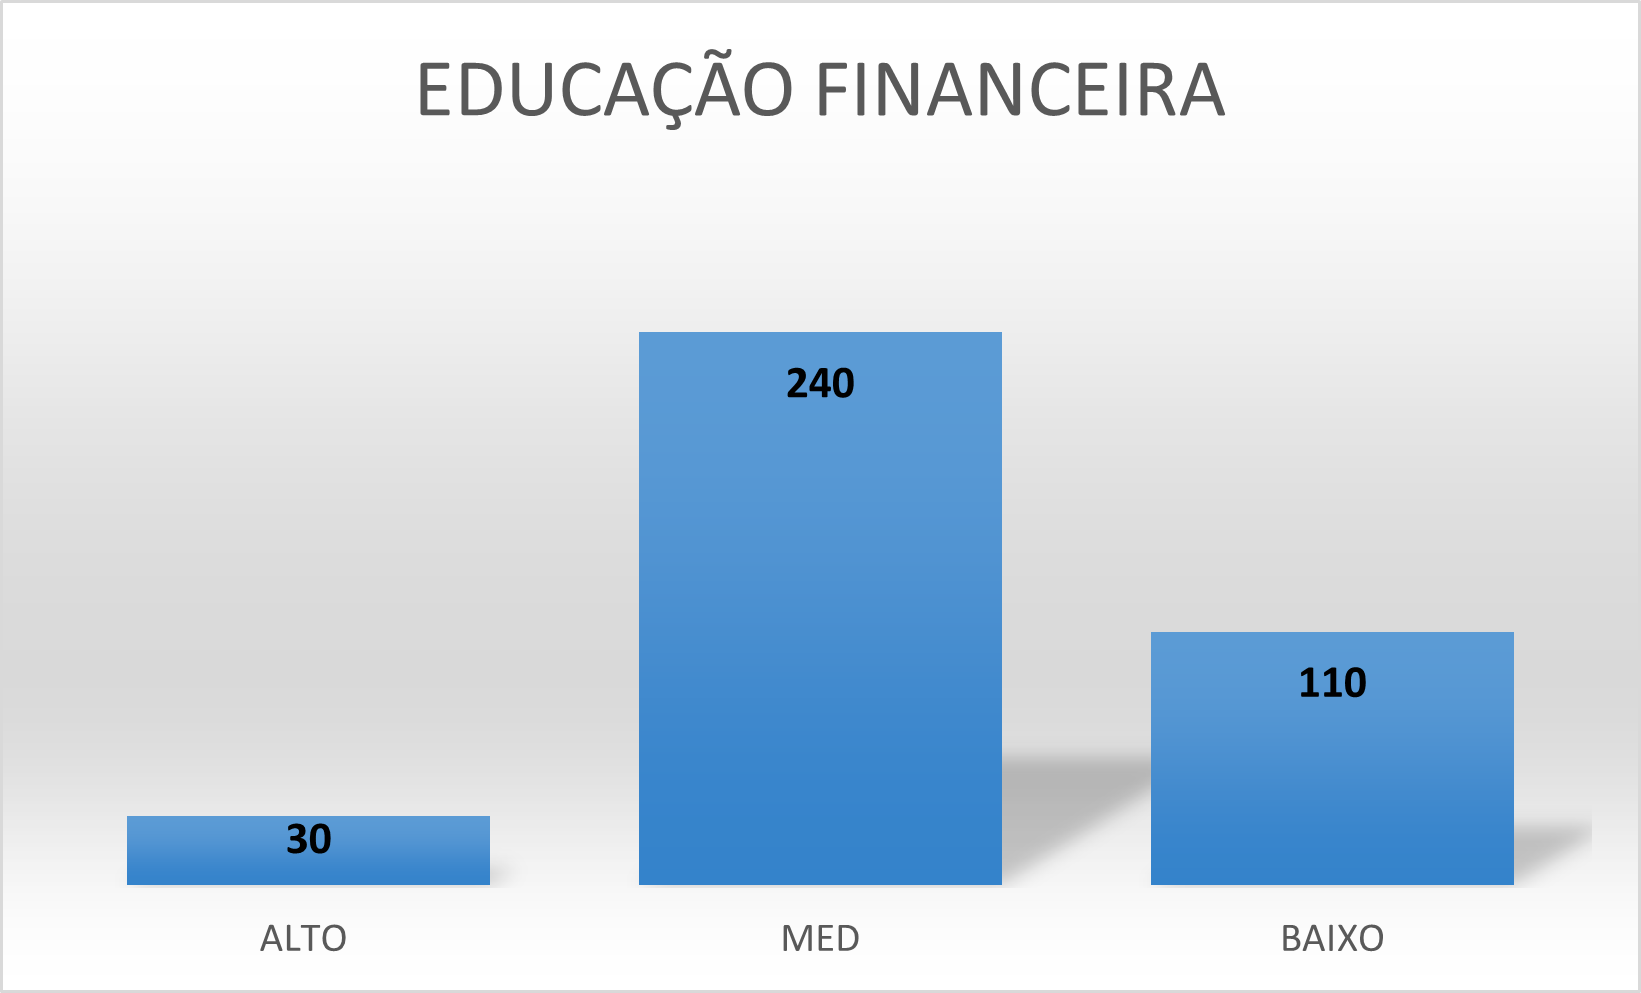
\includegraphics{figs/graph_educacao.png}
            \captionof{figure}{Educação Financeira}
            \label{fig:graph_educacao}
        \end{minipage}       
    \end{center}


    \vspace{\baselineskip}
    \vspace{\baselineskip}
    \vspace{\baselineskip}
    \vspace{\baselineskip}
    \vspace{\baselineskip}
    \vspace{\baselineskip}
    \item Possui Algum Crédito?

    A figura 7 descreve a existência de algum crédito das pessoas respondentes da pesquisa.

    \vspace{\baselineskip}
    \begin{center}
        \begin{minipage}{\textwidth}
            %\centering
            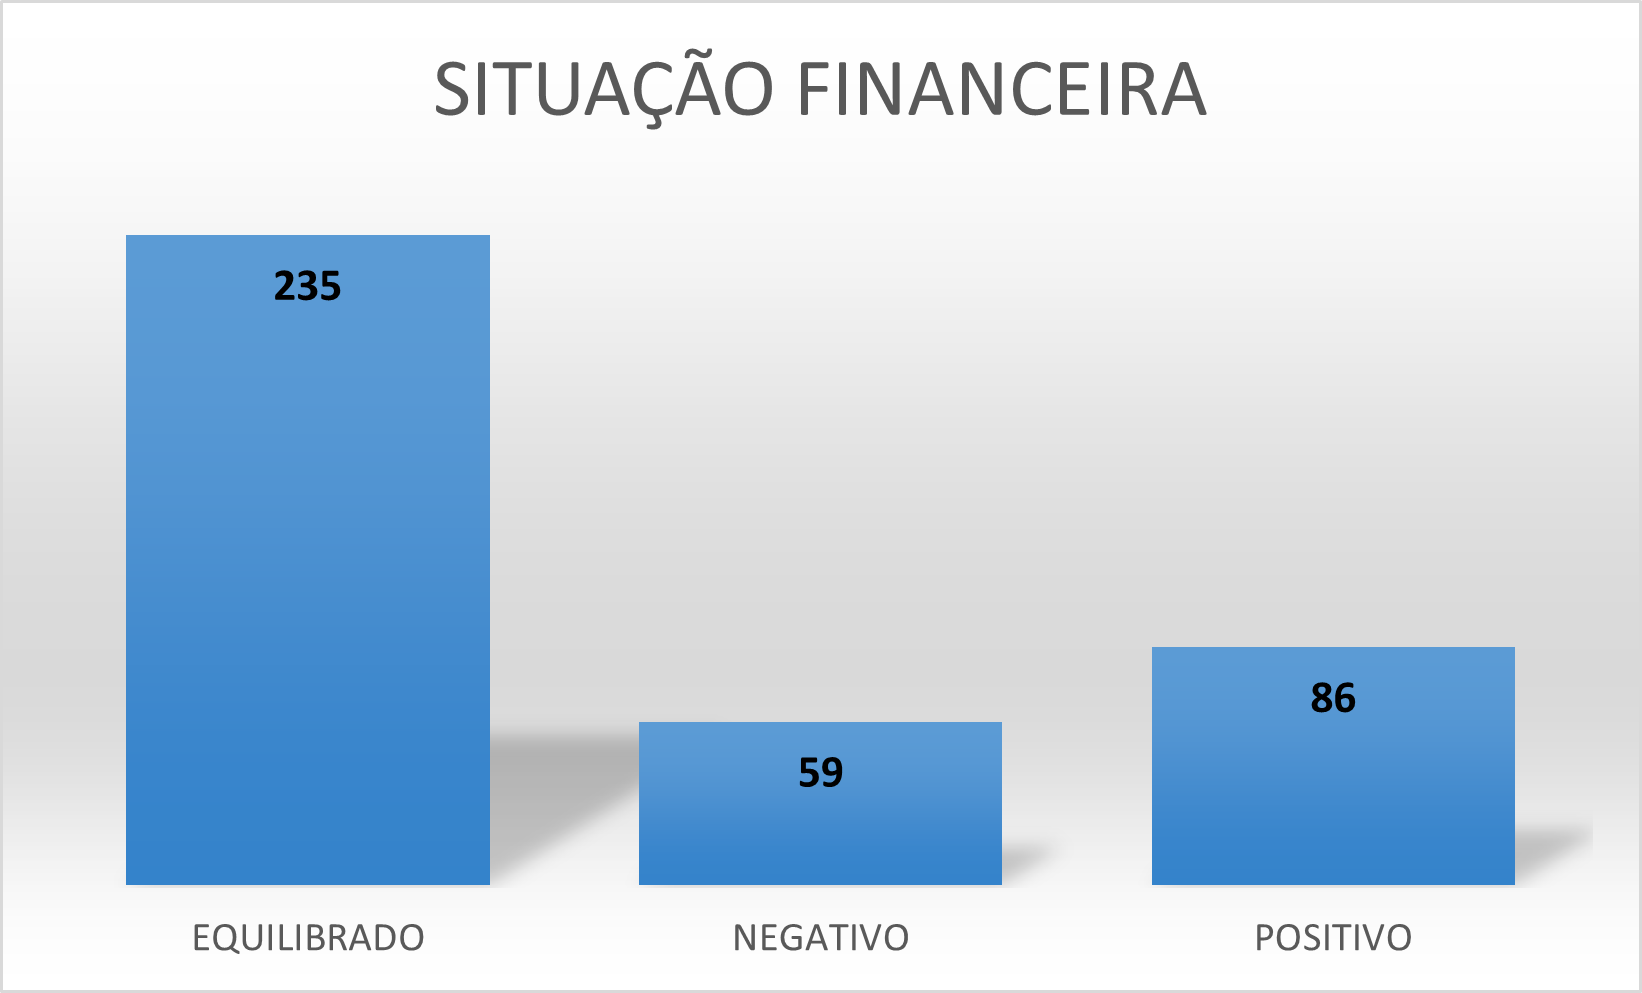
\includegraphics{figs/graph_situacao.png}
            \captionof{figure}{Possui Algum Credito?}
            \label{fig:graph_situacao}
        \end{minipage}        
    \end{center}


    \item Tipo de Crédito

    A figura 8 descreve o tipo de crédito das pessoas respondentes da pesquisa.

    \vspace{\baselineskip}
    \begin{center}
        \begin{minipage}{\textwidth}
            %\centering
            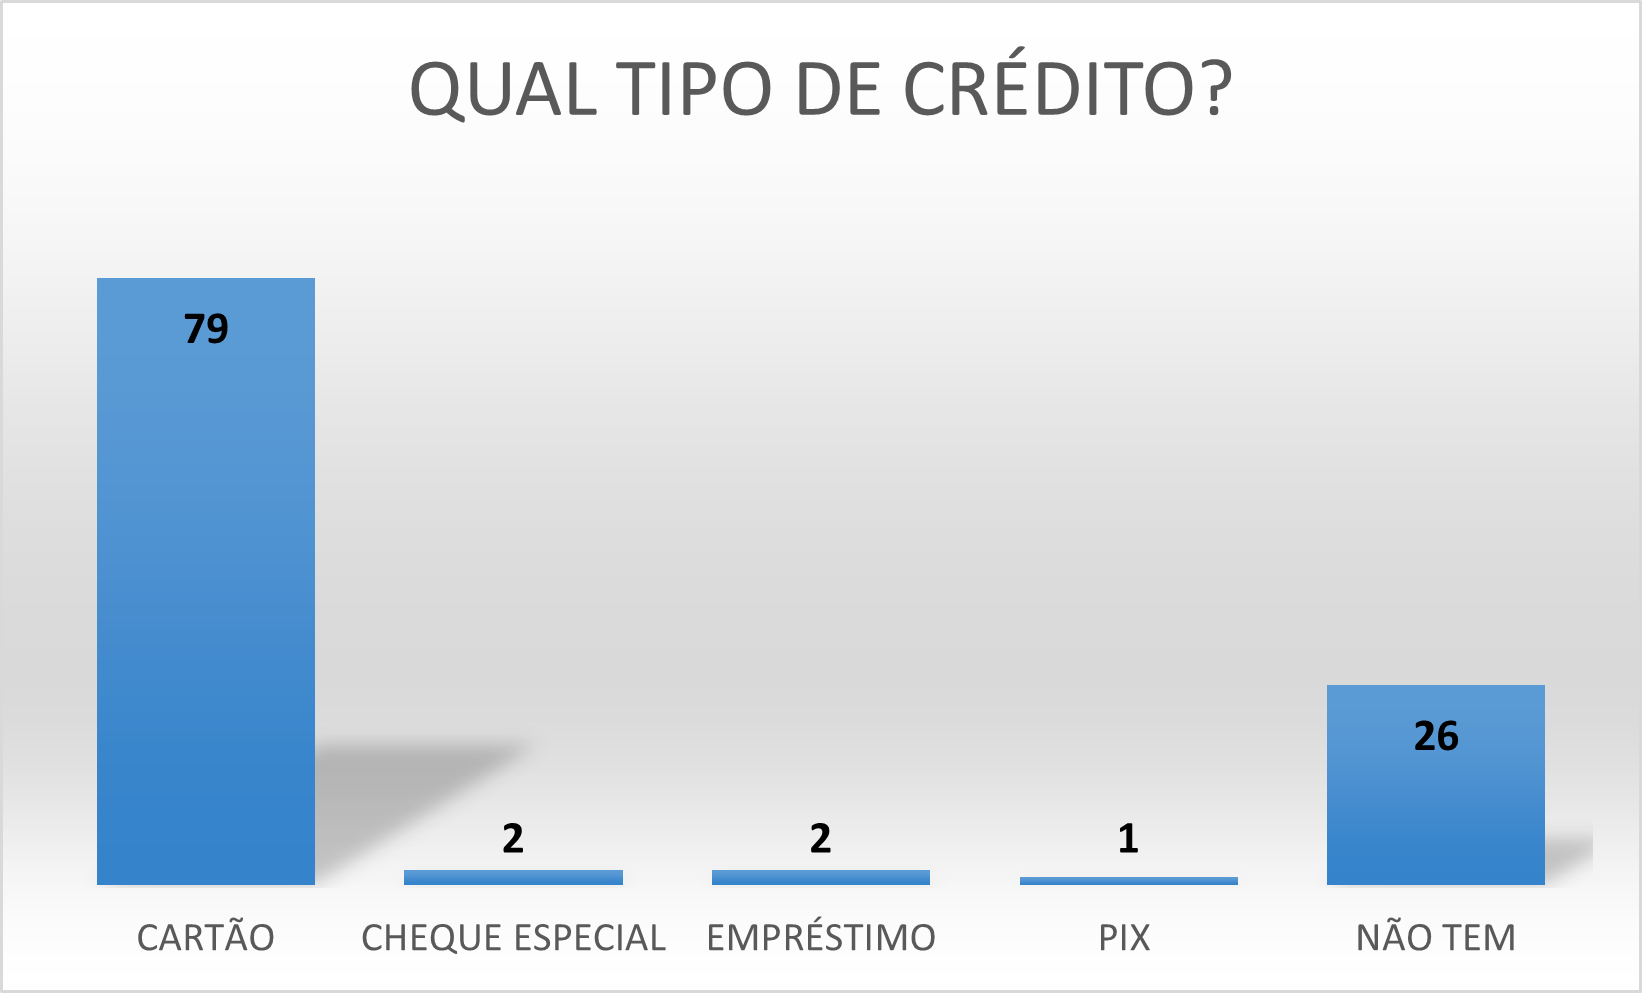
\includegraphics{figs/graph_tipo-credito.png}
            \captionof{figure}{Tipo de Crédito}
            \label{fig:graph_tipo-credito}
        \end{minipage}   
    \end{center}


    \vspace{\baselineskip}
    \vspace{\baselineskip}
    \vspace{\baselineskip}
    \vspace{\baselineskip}
    \item Método Mais Utilizado

    A figura 9 descreve o método mais utilizado das pessoas respondentes da pesquisa.

    \vspace{\baselineskip}
    \begin{center}
        \begin{minipage}{\textwidth}
           %\centering
            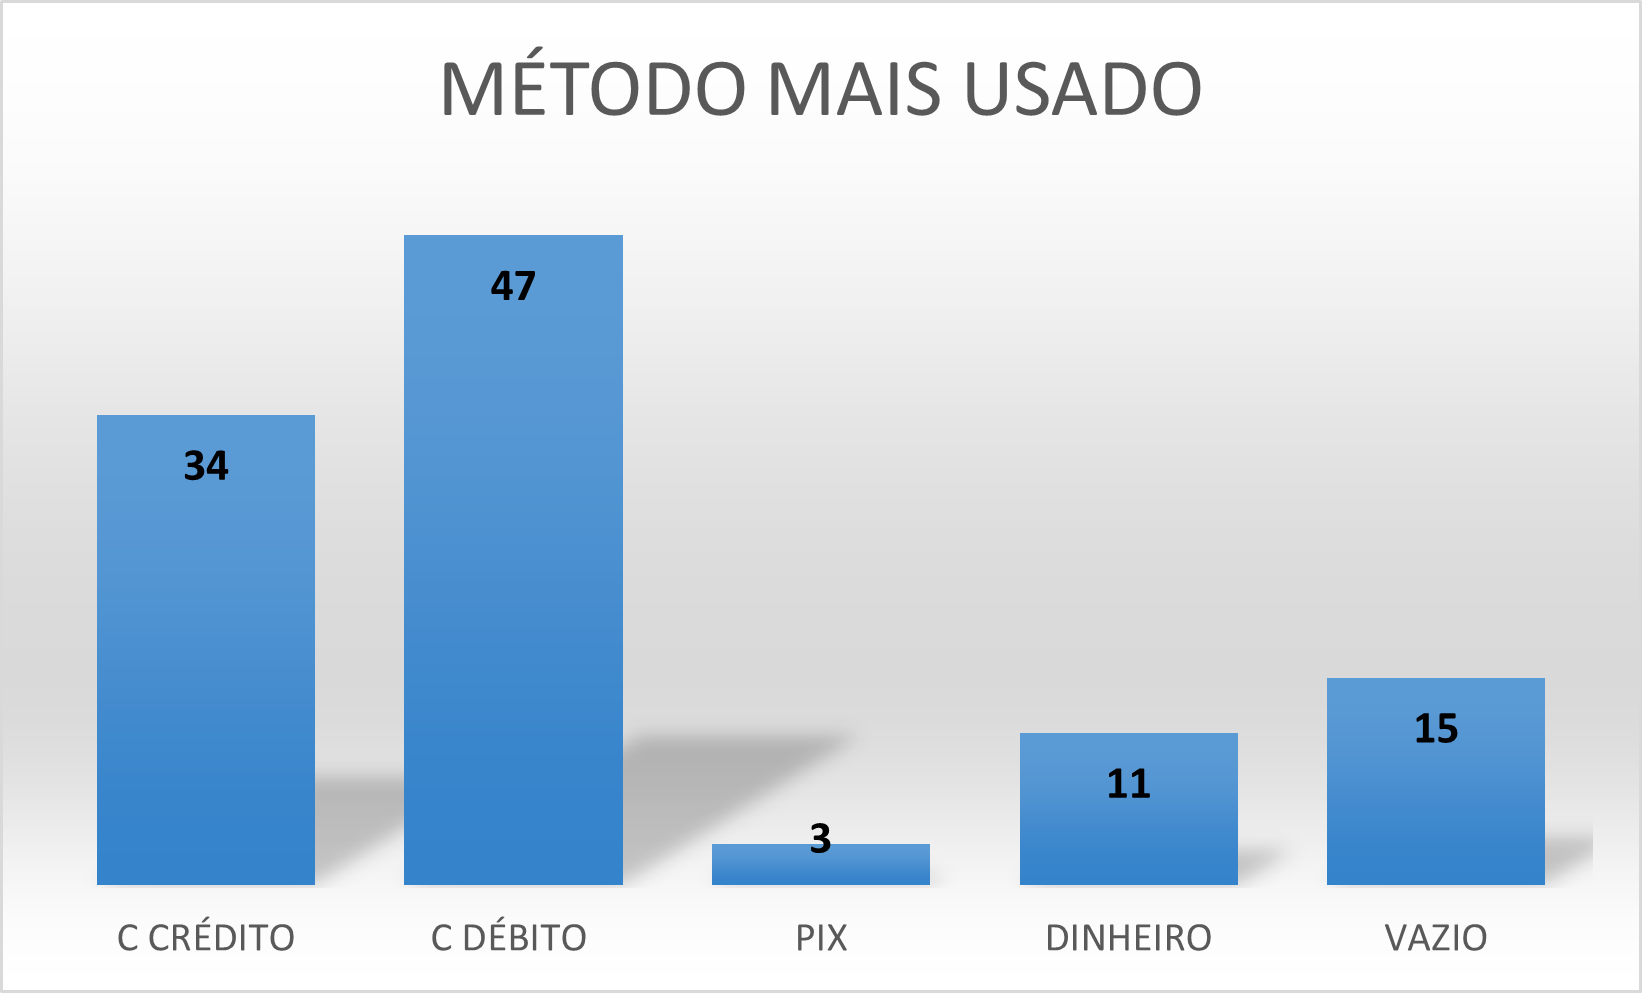
\includegraphics{figs/graph_mais-usado.png}
            \captionof{figure}{ Método Mais Utilizado}
            \label{fig:graph_mais-usado}
        \end{minipage}        
    \end{center}

    \item Se Considera Organizado?

    A figura 10 descreve Se Considera Organizado?, das pessoas respondentes da pesquisa.

    \vspace{\baselineskip}
    \begin{center}
        \begin{minipage}{\textwidth}
            %\centering
            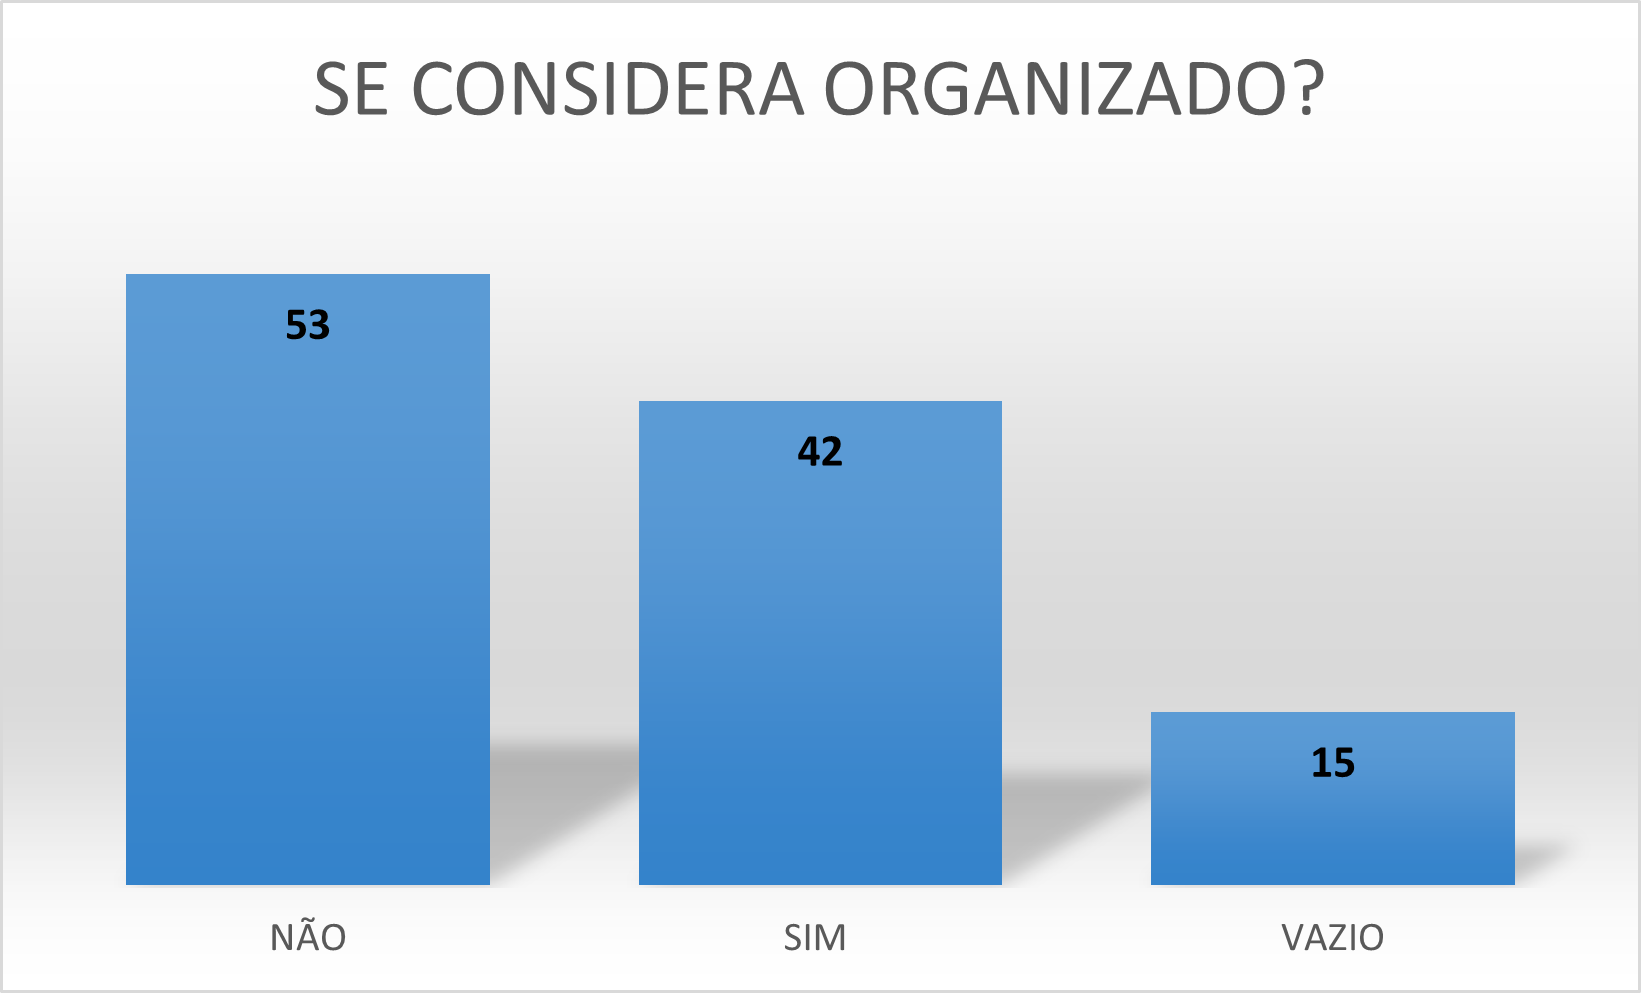
\includegraphics{figs/graph_considera-organizado.png}
            \captionof{figure}{Se Considera Organizado?}
            \label{fig:graph_considera-organizado}
        \end{minipage}        
    \end{center}
    
\end{enumerate}
